\chapter{Multicolor registration}
Biological samples are often labeled with more than one kind of fluorophore to show different structures within the sample. To align the images from
different color channels despite chromatic aberration, beads are used. Beads are
flourophores added to the probe that emit light in all wavelengths the
different markers do, and therefore are visible in all channels. The beads can be
used as landmarks, because their position in the original image is at the same
spot. The task is to find a transformation that maps corresponding beads on each
other.\newline
The aligned images can then be investigated for colocalized structures.\newline
Both tasks can be done using the improved version of the Colorcomposer.

\section{Colorcomposer GUI}
The goal of the colorcomposer tool is to provide software that is easy to use, flexible and powerful. The current version of the colorcomposer is easy to use, because the different channels can be aligned by just selecting the auto align option.\newline
If the user wants to select beads on his or her own, beads can manually be selected and deleted. After the transformation the user can use the implemented tool for colocalization detection or save the transformed images and process them with the tool of his or her choice.\newline
Also the colorcomposer is powerful as it provides information about the number of points currently under the cursor or its intensity. The estimated transformation error and the localization error are computed and stored.\newline
The basic framework for the colorcomposer was set up by \cite{MAJoachim}. It contained the workflow for importing and exporting images the handling of bead objects and a linear transformation that used the beads in the order they were found. This early version was not usable.\newline
Figure \ref{ColorComposer} shows improved colorcomposer GUI with two datasets loaded. The buttons on the right give the user the option to add or remove beads also in addition to the autodetected beads. There are also different sliders to control the values used for bead detection. In the lower right corner there is additional information provided about the total number of points within a rectengular with the selected cursor radius' size. The sum of the intensities and the total number of frames for each data set are also given. This information is helpful to determin whether a cluster of points is a bead or not.\newline
On top there is a menu bar with new options, that enable the user to discard all beads, automatically detect beads, calculate colocalization measures and show or hide the colocalization heatmap.
\begin{figure}
\centering
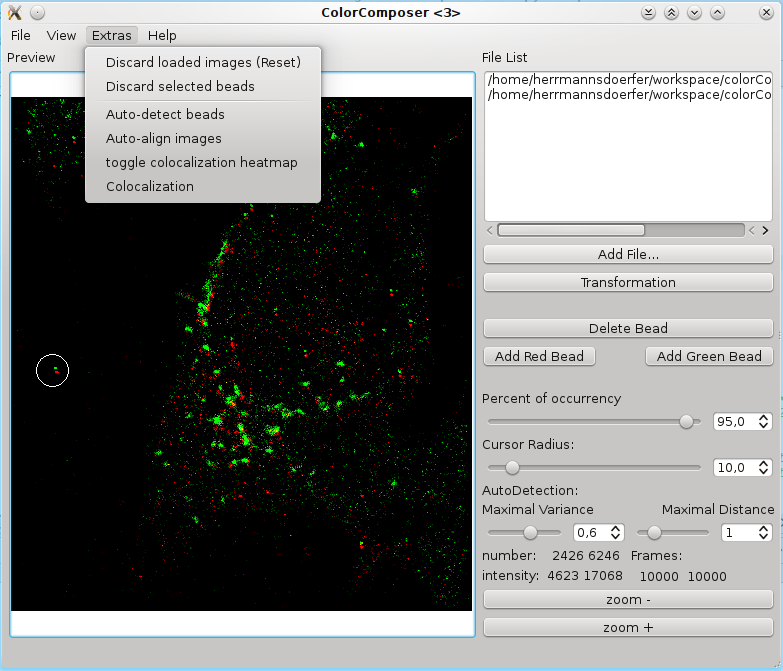
\includegraphics[width = 0.88\textwidth]{pictures/GuiColorcomposer/BeforeAlignmentWithMenu.png}
\caption{Improved colorcomposer GUI. On the right sliders to set the parameters are present. There are also buttons to add or delete single beads. On the lower right additional information about the area under the cursor is displayed, such as numbers of pixels, total intensity and the number of frames in total.}
\label{ColorComposer}
\end{figure}


\section{Features of the colorcomposer application}
\subsection{Invariance of input datas units}
The resulting coordinate files from SimpleSTORM or other STORM algorithms may be given in units of pixels relativly to the unprocessed data or in nanometers. Treating coordinates given in nanometer as pixel units would lead to very huge and very sparse images displayed in the colorcomposer. Therefore the colorcomposer reads out additional information from the coordinates text files header. These informations are the pixel to nanometer ratio and the used factor. With this information the picture can be reconstructed as an upsampled version of the input image by the used factor, regardless of the units used to save the coordinates file. If none of this information is given a pixel to nanometer ratio of 1 is assumed which garantues backward compatibility with older coordinate files given in pixel units.
\subsection{Manual bead selection and removal}
With the improved version of the colorcomposer it is possible to add beads manually. Therefore the desired location is clicked in the preview image and after that either the button "add green bead" or "add red bead" is hit. If there are enough frames containing localizations near the given location a bead is added to the center of mass of the intensities in that area. If the button "delete bead" is pressed all beads in the selected area are deleted.\newline
This feature can be used to add beads missed by the automatic bead detection.
\subsection{Automatic bead detection}
The input for the colorcomposer application is a text file created by the storm
algorithm that contains information about the position, intensity, symmetry,
frame number and signal-to-noise ratio of each detection. The beads should
ideally appear in most of the images. This means they can be found by searching for
detections that appear in almost every frame at the same position.\newline
There was already an automatic bead detection implemented by Joachim Schleicher. This was improved as follows.\newline
All important parameters for the bead detection can now be set in the GUI. The bead detection works by searching for points that appear in most of the frames. Instead of taking all localizations from the first frame as expected bead positions without considering locations that do not appear in the first frame, now a good subset of positions from the first 50 frames by skipping redundant positions based on the minimal distance of a new position to all positions already in the set. The range of 50 frames to look for beads is sufficiant because it is very unlikely that all 50 detections of the bead have been missed.\newline
After good candidates are found their number of points, variance and mean position is determined like described by \cite{MAJoachim}.\newline
In the end beads that are too close are merged to a new bead with its center right between the merged beads.

\subsection{Alignment of two multicolor images}
After the beads for each channel are found, the next task is to find the corresponding
beads in each channel. It happens that some beads only occur in one channel.
If this happens there will be no corresponding bead in the other
channels.\newline
The first step is to discard beads that are far away from any bead of the other color. From the resulting subset of beads the maximal number of possible bead pairs is estimated by taking the smaller number of beads per color.\newline
The iteration begins, which tries to find the best transformation to map all beads from one color to the beads of the other color. Therefore all beads from the color with less beads are chosen and the same number from the other color are selected. This selection is based on
a probabilistic approach and the distance matrix containing the information about the
distances between all beads of the two channels. It is more likely for nearer beads of the other channel to be selected, but any bead within a certain range can be chosen.\newline
Using these pairs of beads, a linear transformation is found, as described by
\cite{MAJoachim}.\newline
This transformation is used to test how many other beads, that were not used to calculate the transformation match intotal. It is assumed that the correct transformation will match other bead pairs in addition. 
This step is repeated multiple times.\newline
The maximal number of matching bead pairs is compared with the number of assumed bead pairs. If less bead pairs are found than expected the number of expected bead pairs is reduced by one and the previous procedure is repeated with the appropriate number of beads randomly chosen from the channel with less beads.\newline
All transformations that match more or equal bead pairs are stored. Also all bead pairs that are aligned under this transformation are stored. The number of assumed bead pairs is reduced by on and the iteration started again. \newline
This loop ends when the assumed number of bead pairs is lower than 3, the minimal number of bead pairs necessary for the calculation of the transformation.\newline
All candidates for the transformation are checked for the occurance of shearing.
In principle shearing should also be allowed for a linear transformation, but tests
indicate that shearing does not occur, so it is disabled to improve stability. \newline 
If there are just
three beads in each channel used for the transformation, then every time a perfect transformation is found,
but the correct one, if possible, is the one without shearing. There will be an other problem with this transformation if the bead density is very high it might be that a transformation with much shearing is found. This compresses the beads of one channel to a slim band. The probability to find a matching point by chance is much greater then. \newline
Figure \ref{badshearing} shows the result of an incorrect transformation of simulated data. The red channel was created by randomly placing beads. The green channel was slightly shifted and rotated. The green channel was transformed to match with the red channel. Just a subset of beads was used to calculate the transformation and so this solution was found and chosen from the algorithm because of the additional matching point.\newline
This effects can be suppressed by not allowing shearing for the transformation.

\begin{figure}
\centering
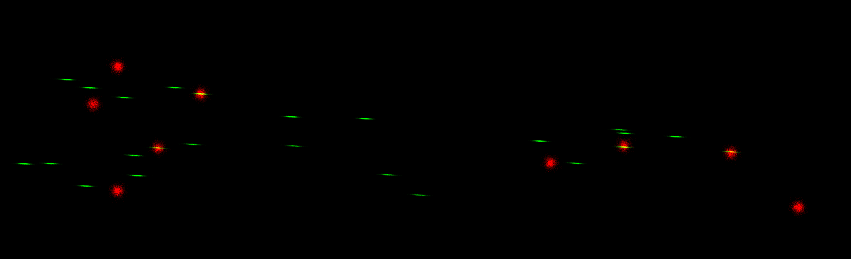
\includegraphics[width = 0.88\textwidth]{pictures/shearingBad.png}
\caption{Affine transformation with shearing enabled. The green channel is deformed and one bead matches by chance which led to selection of this transformation.}
\label{badshearing}
\end{figure}
\subsection{Information about localization certainty}
The detected spots from SimpleSTORM contain some localization error. This error will be derived in section \ref{detectionError}. It depends on the signal-to-noise ratio and the scale of the point spread function of a single fluorophore.

Within all transformations that do not show shearing, the transformation is chosen that has the least root mean square error for all matching pairs of beads.

\section{Total localization error}
There are four contributions to the total localization error considered in this thesis.\newline
First there is the error that arises from the linear transformation to align the beads. To estimate this error the variance of the estimator is used. Since the transformation matrix is calculated by linear regression from the matricies $B$ and $R$ of the localizations of the first and the second layer of beads, with $B$ beeing the matrix of the first layer to that the second layer $R$ is transformed to. The variance of the estimator is
\begin{align}
\text{variance registration}&= \sigma^2 x_0\left(R^TR\right)^{-1}x_0^T, \text{ with }x_0 = \left(x_o,x_1,1\right) \label{gl22}
\end{align}
Using equation \ref{gl22} the variance for all pixel can be calculated.\newline
The second contribution to the total localization error is the localization error of the SimpleSTORM algorithm. Its formula is
\begin{align}
 \text{variance localization} = \frac{N^2\pi}{2S_0^2} \left(1+\frac{\sigma_\text{PSF}^2}{\sigma_\text{filter}^2}\right)^2\left(\sigma_\text{filter}^2+\sigma_\text{PSF}^2\right)^2
\end{align}
It is derived in \ref{detectionError} and can be calculated for each detection individually based on the known signal-to-noise ratio. The signal-to-noise ratio gives directly the signals intensity $S$, because of the known noise variance of one which gives the nois' standard deviation $N$ of also one. The PSFs width was either given or estimated and is passed to the colorcomposer in the detection coordinate file's header along with the prefactor $f$ for the actually used filter. Using this the localization error can be writen as
\begin{align}
 \text{variance localization} &= \frac{N^2\pi}{2S_0^2} \left(1+\frac{\sigma_\text{PSF}^2}{f^2\sigma_\text{PSF}^2}\right)^2\left(f^2\sigma_\text{PSF}^2+\sigma_\text{PSF}^2\right)^2 \\
 &=\frac{N^2\pi}{2S_0^2}\left(1+\frac{1}{f^2}\right)^2\left(1+f^2\right)^2\sigma_\text{PSF}^4\\
 &= \frac{N^2\pi}{2S_0^2}\left(2+\frac{1}{f^2}+f^2\right)^2\sigma_\text{PSF}^4
\end{align}
The third contribution results from the fact that the fluorophors are not directly attached to the sample of interest, but there are the antibodies used for staining inbetween. The upper bound of this error can be estimated under the assumption that the target of the antibodies is much smaller than the antibodies, so that there is no occlusion in the projection. This assumption does not hold in reality. Structures like cell membranes are certainly larger than the antibodies, but the assumption gives an upper bound. 
\begin{align}
\text{var x} &=\frac{1}{\Omega_\text{Sphere}}\int\limits_{\Omega_\text{Sphere}} x^2 dV\\ 
&=\frac{1}{\Omega_\text{Sphere}}\int\limits_0^{2\pi}\int\limits_0^\pi R^2\sin\theta \left(R\cos\phi \sin\theta\right)^2 d\theta d\phi\\
&=\frac{R^2}{4\pi} \int\limits_0^{2\pi}\int\limits_0^\pi \cos^2\phi \sin^3\theta d\theta d\phi\\
&=\frac{R^2}{4\pi} \left[\frac{1}{2}\phi +\frac{1}{4}\sin 2\phi \right]_0^{2\pi}\int\limits_0^\pi \sin^3\theta d\theta \\
&=\frac{ R^2}{2} \left[\frac{1}{12}\cos3\theta -\frac{3}{4}\cos\theta \right]_0^\pi\\
&=\frac{2}{3} R^2
\end{align}
$R$ is the assumed distance of the fluorophore to the structure it is attached to.\newline
The fourth and minor contribution to the total localization error for each pixel is the quantization noise. It occurs when continous intensities, as the photons forming the PSF, are transformed into integer values. Quantisation noise describes the round-off error. The round-off error can be any value between -0.5 and 0.5 and is uniformly distributed. Its variance $\sigma_Q^2$ is
\begin{align}
 \sigma_Q^2 =\int\limits_{-\frac{1}{2}}^{\frac{1}{2}} x^2 dx = \frac{1}{12}
\end{align}
The unit of this error is the pixel size of the upscaled image and therefore more and more negligible the higher the upscaling factor is.\newline
To get the total localization error all four variances are summed up for each pixel.

\section{Colocalization}
Colocalization in wide field microscopy is a measure of the overlap of data point from different channels. It can provide information whether or not two molecules interact. With increasing resolution of the images colocalization becomes more and more a measure of similar structures near each other. Two structures can't be at the very same position in the cell. The colorcomposer software provides both global and local colocalization measurements.
\subsection{Global colocalization}
The most common colocalization measure is Pearsons correlation coefficient \cite{pearson}. It is given as:
\begin{align}
\text{Pearson correlation coefficient =}\frac{\sum ^n _{i=1}(X_i - \bar{X})(Y_i - \bar{Y})}{\sqrt{\sum ^n _{i=1}(X_i - \bar{X})^2} \sqrt{\sum ^n _{i=1}(Y_i - \bar{Y})^2}}
\end{align}
It is the ratio between the covariance between the points of two channels and their standard deviation.\newline

Also the Manders correlation coefficients $M_1$ and $M_2$ and the overlap coefficient (\cite{manders}) are calculated. Two channels a red and a green one is assumed.
\begin{align}
M_1 =& \frac{\sum_i R_{i,\text{coloc}}}{\sum_i R_i}&M_2 = & \frac{\sum_i G_{i,\text{coloc}}}{\sum_i G_i}
\end{align}
With $R_{i,\text{coloc}} = R_i$ if $G_i >0$ and $R_{i,\text{coloc}} = 0$ otherwise and $G_{i,\text{coloc}} = G_i$ if $R_i >0$ and $G_{i,\text{coloc}} = 0$. $G_i$, $R_i$ are the intensities of the pixel of the green and red channel.
\begin{align}
\text{overlap coefficient} = \frac{\sum_i R_i \cdot G_i}{\sqrt{\sum_i \left(R_i\right)^2 \cdot \sum_i \left(G_i\right)^2}}
\end{align}

\subsection{Local colocalization}
Global colocalization has the drawback that there is just one value for the whole image, not yielding any information about where colocalization is localised. If there are regions in the image that show much colocalization and other regions without colocalization the same colocalization coefficient might be achieved as if one channel is distributed randomly.\newline
For local colocalization analysis the algorithm from \cite{coloc} is used and was further developed to gain a speed boost. The algorithm runs approximatly 40 times faster now. This was achieved by using scipys (\cite{scipy}) ckdtree function, which is a k-d tree implemented in C.\newline
The concept of the localization algorithm is to compute a colocalisation value for each coordinate. This is done by calculating the distribution of all detections of both channels around each detection within a maximal radius $R$. This maximal radius determins the longest distance for which colocalization can be detected.\newline

Figures \ref{radius50} and \ref{radius100} show the results from the colocalization calculation for both the red and green channel from \ref{cropedOrig}. The difference between \ref{radius50} and \ref{radius100} is that the maximal distance is larger for the later. This example shows the larger the maximal distance the more colocalization is detected. This choice for the maximal distance depends strongly on the sample.





%\subsection{Validation of colocalization approaches}
%"Image set CBS001RGM-CBS010RGM from the Colocalization Benchmark Source
%(www.colocalization-benchmark.com) was used to validate colocalization."

\begin{figure}
\begin{minipage}[t]{0.99\textwidth}
\centering
	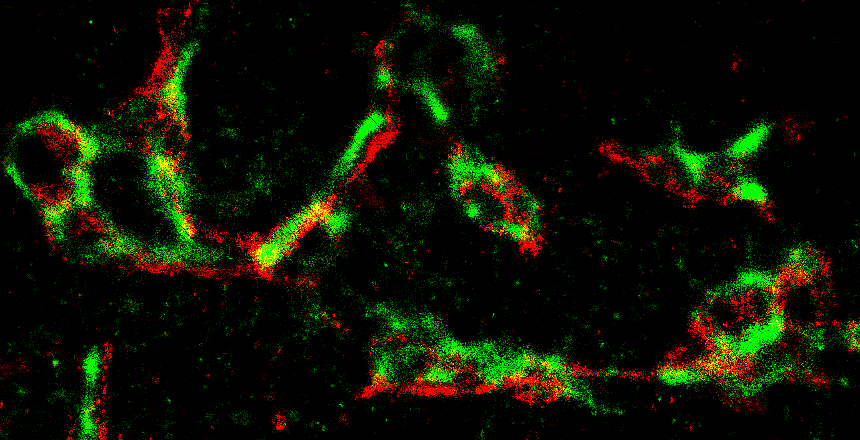
\includegraphics[width = 0.8\textwidth]{pictures/colocalization/cropedOrig.png}
	\caption{Aligned image showing colocalization.}
	\label{cropedOrig}	
\end{minipage}\\
\begin{minipage}[t]{0.99\textwidth}
\subfloat[]{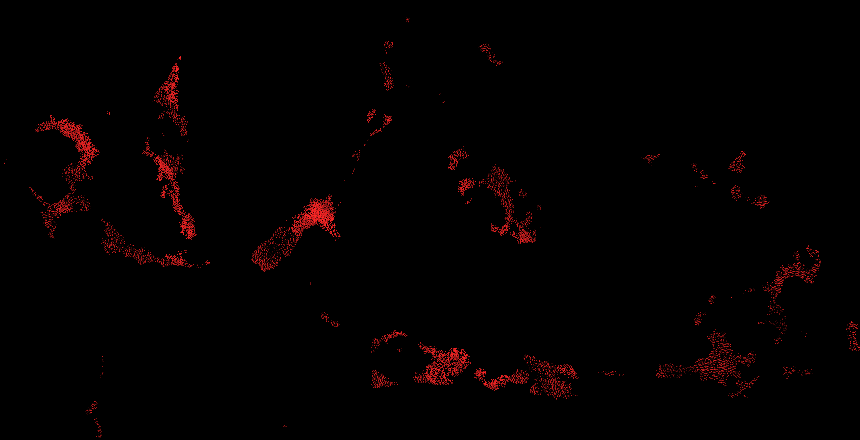
\includegraphics[width = 0.485\textwidth]{pictures/colocalization/cropedCh0.png}}\hfill
\subfloat[]{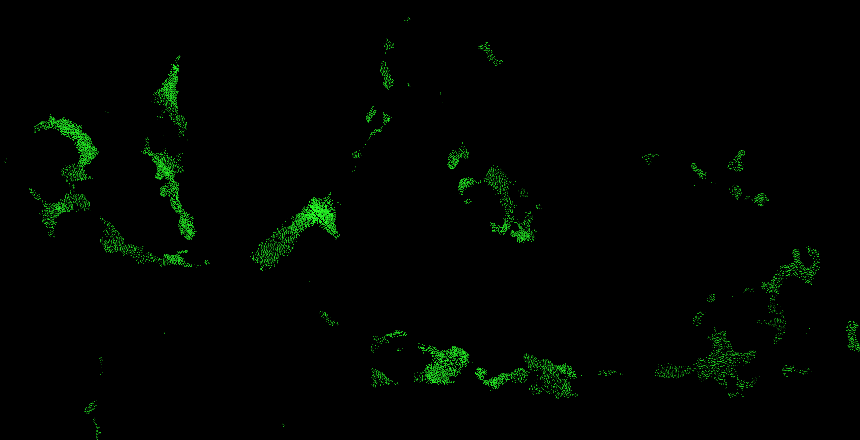
\includegraphics[width = 0.485\textwidth]{pictures/colocalization/cropedCh1.png}}
	\caption{Colocalization for the red and green channel with a maximal radius $R=50$ nm}
	\label{radius50}	
\end{minipage}\\
\begin{minipage}[t]{0.99\textwidth}
\subfloat[]{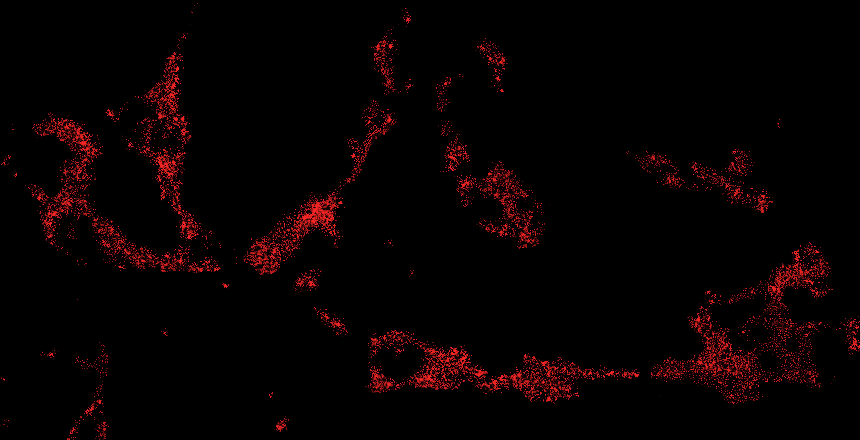
\includegraphics[width = 0.485\textwidth]{pictures/colocalization/cropedCh0100.png}}\hfill
\subfloat[]{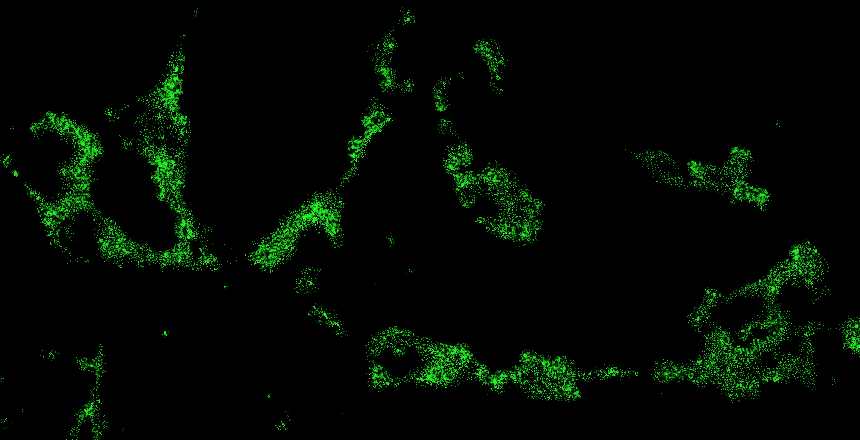
\includegraphics[width = 0.485\textwidth]{pictures/colocalization/cropedCh1100.png}}
	\caption{Colocalization for the red and green channel with a maximal radius $R=100$ nm}
	\label{radius100}	
\end{minipage}
\end{figure}